
\documentclass[conference]{IEEEtran}
\IEEEoverridecommandlockouts
% The preceding line is only needed to identify funding in the first footnote. If that is unneeded, please comment it out.
\usepackage{cite}
\usepackage{amsmath,amssymb,amsfonts}
\usepackage{algorithmic}
\usepackage{graphicx}
\usepackage{textcomp}
\usepackage{xcolor}
\def\BibTeX{{\rm B\kern-.05em{\sc i\kern-.025em b}\kern-.08em
    T\kern-.1667em\lower.7ex\hbox{E}\kern-.125emX}}
\begin{document}

\title{Revolutionizing System Support: Supporting Firecracker Virtualization for Jinux Platform\\
{\footnotesize \textsuperscript{*}Group project I - Presentation I}
\thanks{}
}

\author{\IEEEauthorblockN{1\textsuperscript{st} Ruixiang JIANG}
\IEEEauthorblockA{\textit{Southern University of Science and Technology} \\
Shenzhen, China \\
12111611@mail.sustech.edu.cn}
\and
\IEEEauthorblockN{2\textsuperscript{nd} Wenqian YAN}
\IEEEauthorblockA{\textit{Southern University of Science and Technology} \\
Shenzhen, China \\
12113020@mail.sustech.edu.cn}
}

\maketitle

\begin{abstract}
Firecracker is an open-source virtualization technology developed by Amazon Web Services (AWS), tailored for the modern cloud computing landscape. At the same time, Jinux is a secure, fast, and general-purpose OS kernel, written in Rust and providing Linux-compatible ABI. Our propose is to support Firecracker virtualization for Jinux platform.
\end{abstract}

\begin{IEEEkeywords}
Firecracker, Jinux, Rust
\end{IEEEkeywords}

\section{Introduction}
Firecracker, an open-source virtualization technology, has been meticulously engineered by Amazon Web Services (AWS) to cater to the evolving needs of the contemporary cloud computing ecosystem. Its design is characterized by a set of intricate features and optimizations that enable efficient virtualization and rapid deployment of virtual machines (VMs).

In parallel, Jinux, an exceptionally secure and high-performance operating system kernel written in the Rust programming language, boasts full compatibility with the Linux-compatible Application Binary Interface (ABI). Jinux's reputation for security and speed makes it an ideal candidate for enhancing the virtualization landscape.

Our primary research objective is to advance the compatibility and seamless integration of Firecracker virtualization within the Jinux platform. This collaboration will involve detailed analysis, testing, and the development of necessary interfaces and components. By bringing together the strengths of Firecracker and Jinux, we aim to deliver a robust and secure virtualization environment that not only meets the stringent demands of cloud computing but also fosters innovation in the field of virtualization technology.

\section{Distinctive  Characteristics  of  Firecracker}
In the era of cloud computing, the demand for fast and efficient virtualization solutions has grown exponentially. Firecracker, introduced by AWS, offers a unique approach to meet these demands. 

\begin{figure}[htbp]
\centering
\includegraphics [width=0.8\linewidth]{FirecrackerBig.png}
\caption{Firecracker architecture \& server setup\cite{b1}}
\label{fig}
\end{figure}

Firecracker provides a RESTful API through which a user can change some settings of the virtual machine. Because of its direct interaction with a user, the API server component is a good choice for our set of targets.

The guest OS must interact with the hypervisor virtual devices for access to network and storage. A custom operating system crafted by a malicious user can use this communication link as an attack vector. Currently, in Firecracker only five emulated devices are available: (i) a network device, (ii) a block device, (iii) a vsock implementation, (iv) a serial console, and (v) a minimal keyboard controller. This seems to be a substantial attack surface, and we chose to focus our attention on the first three devices as they provide a complex implementation that is prone to hidden vulnerabilities.\cite{b4}

\subsection{Rapid Boot Time}
One of the standout features of Firecracker is its remarkable speed in launching virtual machines. With a startup time of less than one second, Firecracker is ideally suited for applications requiring rapid scaling, such as serverless functions.

There is a comparison of the boot times of different VMMs. The boot time is measured as the time between when VMM process is forked and the guest kernel forks its init process. For this experiment we use a minimal init implementation, which just writes to a pre-configured IO port. We modified all VMMs to call exit() when the write to this IO port triggers a VM exit.\cite{b5}

The figure below shows the cumulative distribution of (wall-clock) kernel boot times for 500 samples executed serially, so only one boot was taking place on the system at a time. Firecracker results are presented in two ways: end-to-end, including fork- ing the Firecracker process and configuration through the API; and pre-configured where Firecracker has already been set up through the API and time represent the wall clock time from the final API call to start the VM until the init process gets executed.\cite{b5}

\begin{figure}[htbp]
\centering
\includegraphics [width=0.8\linewidth]{time1.png}
\caption{Cumulative distribution of wall-clock times for start- ing MicroVMs in serial, for pre-configured Firecracker (FC- pre), end-to-end Firecracker, Cloud Hypervisor, and QEMU.\cite{b5}}
\label{fig_time1}
\end{figure}

This feature enables cloud providers to allocate resources dynamically, improving the overall user experience and resource utilization. Firecracker can achieve rapid boot time primarily due to its lightweight and minimalistic design, which eliminates many of the traditional virtualization overheads.

Here are the key reasons why Firecracker can provide such fast boot time below.
\begin{itemize}
	\item MicroVM Architecture\\
		Firecracker uses a MicroVM (micro virtual machine) architecture. Unlike traditional VMs, MicroVMs are stripped down to include only essential components required for execution. This minimalistic approach reduces the time needed for the VM to start, as there are fewer services and processes to initialize.
	\item Firecracker Kernel\\
		Firecracker uses the Firecracker kernel, which is a custom-built, minimalistic and highly optimized Linux kernel tailored specifically for lightweight VMs. This specialized kernel is designed to boot quickly and manage VMs efficiently.
	\item Just-In-Time Initialization\\
		Firecracker employs a just-in-time initialization process, meaning that many VM components and services are initialized only when they are first used. This defers the startup of non-essential components until they are required, speeding up the initial VM launch.
	\item Pre-Allocated Resources\\
		Firecracker pre-allocates resources for VM instances, which eliminates the need for resource-intensive operations like dynamic memory allocation during boot-up. This approach reduces boot time by ensuring that the VM has immediate access to the resources it needs.
	\item Reduced Emulation Overhead\\
		Firecracker uses a KVM (Kernel-based Virtual Machine) backend, which allows it to leverage hardware virtualization support. This results in significantly reduced CPU and memory overhead compared to full virtualization, further contributing to faster boot time.
	\item Single-Purpose VMs\\
		Firecracker is designed for single-purpose VMs, such as serverless functions or container instances, which means it doesn't need to load a full-fledged operating system and associated services, further reducing startup time.
\end{itemize}
These design principles, along with a focus on simplicity and efficiency, enable Firecracker to achieve rapid boot time, making it well-suited for use cases where fast scalability and low latency are essential, such as serverless computing and containerization.

\subsection{Resource Efficiency}
Firecracker is designed with resource efficiency in mind. It utilizes a minimalistic approach to virtual machine management, resulting in lower resource overhead. This efficient resource usage allows for the deployment of numerous VM instances on the same physical host, increasing the density of workloads without sacrificing performance. It achieves resource efficiency through several design choices and optimizations that minimize resource overhead.
\begin{itemize}
	\item Low Memory Footprint\\
		Firecracker's custom-built kernel and minimalistic design contribute to a small memory footprint for each VM. This reduction in memory usage allows for increased VM density on the same host, optimizing resource utilization.
	\item Multi-Tenant Isolation\\
		Firecracker's strong isolation mechanisms ensure that each VM is securely isolated from others, preventing resource contention and interference in multi-tenant environments.
	\item Resource C-group Management\\
		Firecracker uses resource control mechanisms like C-groups to manage resource allocation to VMs. Administrators can set resource limits and priorities, enabling fine-grained resource management and optimization.
	\item Efficient Component Initialization\\
		Firecracker employs a just-in-time initialization process to activate VM components and services only when they are needed. This design minimizes resource usage during VM boot-up, ensuring efficient resource allocation.
\end{itemize}
These resource-efficient design principles make Firecracker an excellent choice for cloud environments where efficient resource usage and scalability are crucial, as it allows for the efficient execution of workloads without compromising on performance or security.

\subsection{High security}
Firecracker emphasizes security in its design to provide a secure virtualization environment. The following features and design principles contribute to Firecracker's security.
\begin{itemize}
	\item Isolation\\
		Firecracker ensures strong isolation between VM instances. Each VM runs in its own isolated environment, and there is limited interaction between VMs. This isolation helps prevent security breaches and resource interference. What's more, it isolates VMs from the underlying host system, limiting the impact of potential attacks on the host. The attack surface presented to the host is minimized, enhancing overall system security.
	\item Minimal Attack Surface\\
		Firecracker's minimalist design reduces the attack surface. By stripping away unnecessary components and services, it decreases the potential entry points for attackers.
	\item Customizable Security Policies\\
		Firecracker allows administrators to customize security policies to meet their specific requirements. This flexibility enables the implementation of security controls tailored to the needs of a given environment.
	\item Monitoring and Auditing\\
		Firecracker can be integrated with monitoring and auditing tools to track VM activities and detect any suspicious behavior or security breaches. This proactive approach enhances overall security.
\end{itemize}
By incorporating these security features and design principles, Firecracker offers a secure virtualization platform, making it suitable for multi-tenant environments, critical workloads, and scenarios where strong security is a top priority.

\subsection{Container Support}
Firecracker complements containerization technologies like Docker and Kubernetes. It enables the quick encapsulation of containers into virtual machines, delivering improved isolation and security. This integration allows organizations to leverage the benefits of both containerization and virtualization for their workloads.

In conclusion, Firecracker represents a significant advancement in the field of virtualization, offering a host of compelling advantages for the modern cloud computing landscape. Its ability to deliver rapid boot time, resource efficiency, security, and container support positions it as a versatile and impactful solution for a wide range of cloud-based workloads and applications.

The rapid boot time of Firecracker, measured in milliseconds, is a game-changer in the dynamic world of cloud computing. This feature allows cloud providers to allocate resources dynamically and respond to varying levels of demand with unmatched agility. Whether in the context of serverless computing, microservices, or container orchestration, this quick provisioning capability ensures a responsive user experience and maximizes resource utilization.

Resource efficiency is another pillar of Firecracker's strength. Its MicroVM architecture and pre-allocation of resources not only reduce overhead but also enable multiple virtual machine instances to coexist harmoniously on the same hardware, thereby optimizing infrastructure utilization. This trait is especially relevant in cloud environments where resource efficiency can translate into substantial cost savings.

Security is a paramount concern in the cloud, and Firecracker addresses it admirably. By isolating each virtual machine, limiting the attack surface, and reducing the risk of resource contention, Firecracker fortifies the security posture of cloud-based workloads. In multi-tenant environments, these security features enhance overall system integrity and data protection.

As an open-source project, Firecracker fosters collaboration, innovation, and transparency. It empowers developers to customize and extend the technology to meet specific use cases, thus contributing to the ongoing evolution of the virtualization landscape.

Furthermore, Firecracker's seamless integration with container technologies such as Docker and Kubernetes provides an extra layer of isolation and security for containerized workloads. This compatibility allows organizations to harness the advantages of both containerization and virtualization, striking a harmonious balance between agility and security.

In a rapidly evolving cloud computing landscape, Firecracker's blend of rapid provisioning, resource efficiency, security, and container support makes it an invaluable tool. It accommodates the requirements of a diverse array of applications, from serverless functions to microservices, and ensures that cloud environments remain responsive, secure, and cost-effective. The dynamic interplay between these advantages positions Firecracker as a key enabler of innovation and efficiency in the digital era.

\section{Distinctive  Characteristics  of  Jinux}

Briefly, Jinux is a secure, fast, and general-purpose OS kernel, written in Rust and providing Linux-compatible ABI.\cite{b2}

Jinux stands out in its commitment to the principle of least privilege while concurrently maintaining high performance standards. This distinctive approach is underpinned by the comprehensive utilization of the Rust programming language, which, in contrast to conventional system programming languages such as C/C++, boasts an array of exceptional attributes. These attributes encompass an expressive type system, memory safety with the option of unsafe extensions, versatile macros, and a customizable toolchain. By harnessing the intrinsic capabilities of Rust, Jinux successfully architects zero-cost abstractions that facilitate the enforcement of the principle of least privilege across three distinct levels, thereby enhancing both security and performance.
\begin{itemize}
	\item The architectural level.\\
		Jinux is architected as a framekernel, where the entire OS resides in a single address space and unsafe Rust code is restricted to a tiny portion of the OS called Jinux Framework. The Framework exposes safe APIs to the rest of Jinux, which implements the most of OS functionalities in safe Rust code completely. Thanks to the framekernel architecture, Jinux's TCB for memory safety is minimized.

\begin{figure}[htbp]
\centering
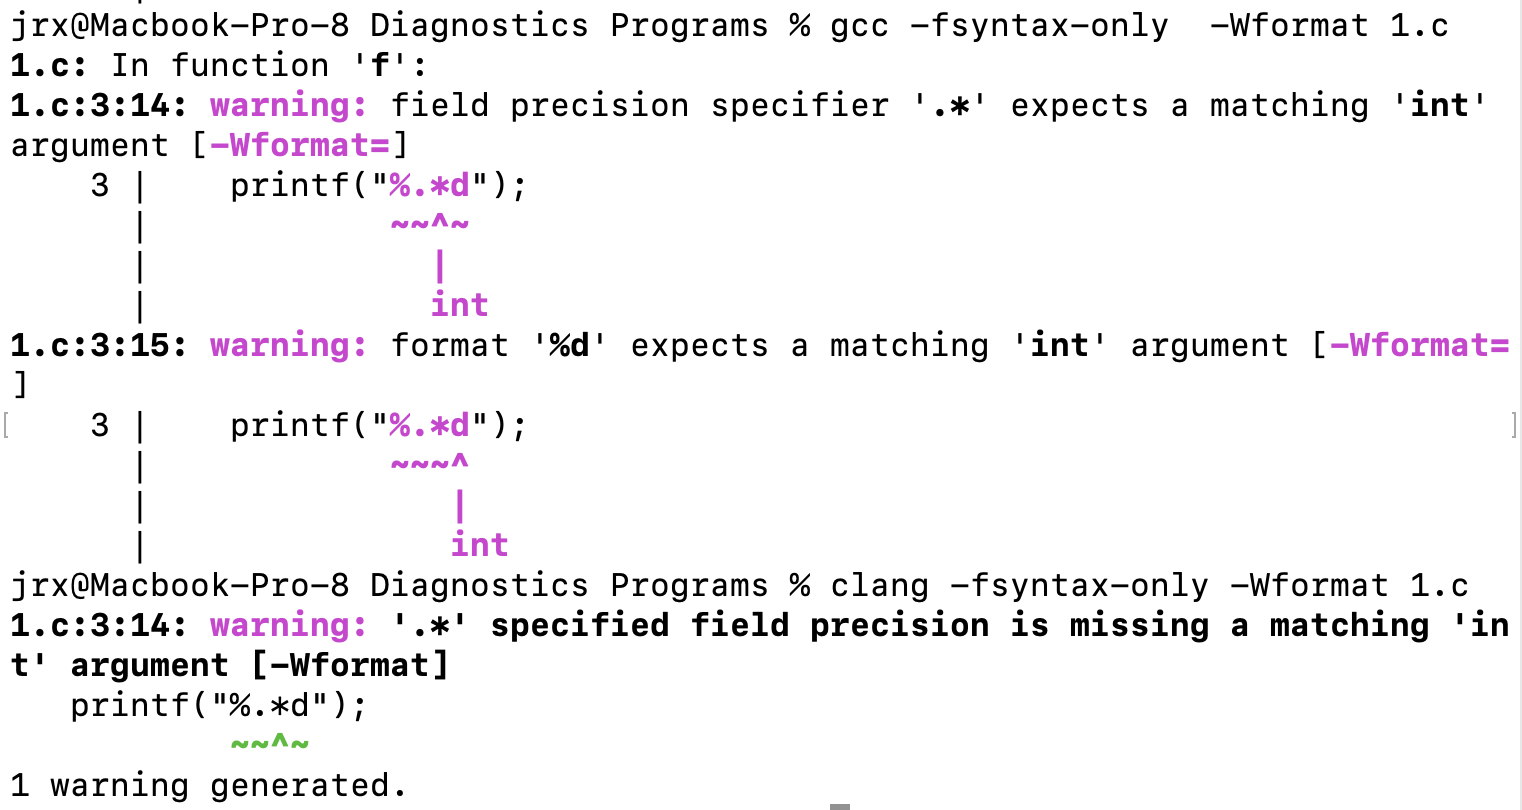
\includegraphics [width=0.8\linewidth]{1.png}\\
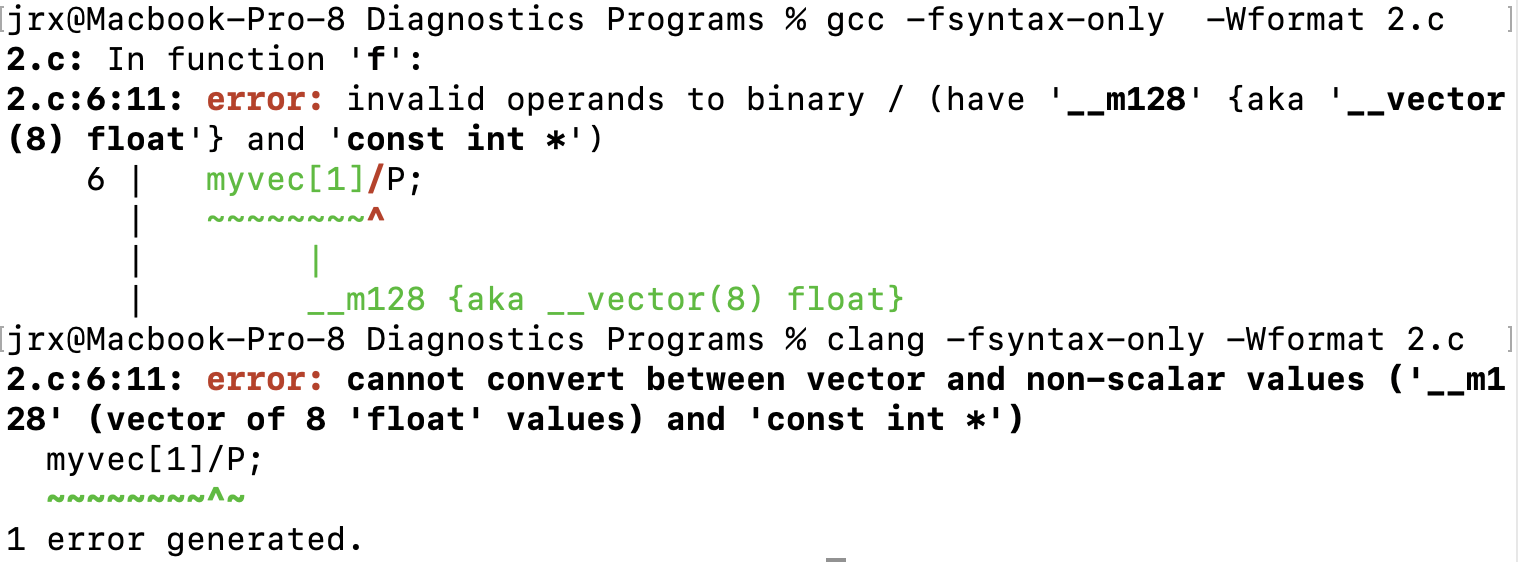
\includegraphics [width=0.8\linewidth]{2.png}
\caption{A comparison between the architectures of traditional OSes and KxOS}
\label{fig}
\end{figure}

	\item The component level.\\
		Upon Jinux Framework is a set of OS components, each of which is responsible for a particular OS functionality, feature, or device. These OS components are Rust crates with two traits: (1) containing safe Rust code, as demanded by the framekernel architecture, and (2) being governed by Jinux Component System, which can enforce a fine-grained access control to their public APIs. The access control policy is specified in a configuration file and enforced at compile time, using a static analysis tool.

	\item The object level.\\
		Jinux promotes the philosophy of everything-is-a-capability, which means all kernel resources, from files to threads, from virtual memory to physical pages, should be accessed through capabilities. In Jinux, capabilities are implemented as Rust objects that are constrained in their creation, acquisition, and usage. One common form of capabilities is those with access rights. Wherever possible, access rights are encoded in types (rather than values) so that they can be checked at compile time, eliminating any runtime costs.\cite{b2}
\end{itemize}

Here is an overview of the architecture of Jinux.

\begin{figure}[htbp]
\centering
\includegraphics [width=0.8\linewidth]
	{archOverview.png}
\caption{An overview of architecture of Jinux\cite{b3}}
\label{fig}
\end{figure}

Security is at the core of Jinux's design philosophy. The operating system adopts the ``least privilege principle" as its guiding security best practice. This principle ensures that each component of the system has the minimum access and permissions required to perform its function, reducing the potential attack surface. Jinux enforces this principle by dividing itself into two distinct halves: a privileged OS core and unprivileged OS components. What sets Jinux apart is its use of Rust, a programming language known for its focus on memory safety and strong guarantees. While all OS components are written entirely in safe Rust, only the privileged OS core is allowed to incorporate unsafe Rust code. This careful separation of responsibilities enhances the system's security, reducing the risks associated with common programming errors and vulnerabilities. Additionally, Jinux introduces the concept of "everything-is-a-capability." Capabilities are elevated to the status of a ubiquitous security primitive used throughout the OS. Advanced features of Rust, such as type-level programming, are harnessed to make capabilities more accessible and efficient. The result is a robust security infrastructure that not only improves the system's resilience but also maintains its performance.

OS-level virtualization is a powerful tool for creating lightweight and efficient container environments. However, concerns have arisen regarding the security of containers, particularly when compared to traditional virtual machines. Malicious containers may exploit privilege escalation vulnerabilities in the underlying OS kernel, posing a threat to the host system. To address this issue, Jinux seeks to establish itself as a trustworthy OS-level virtualization platform. It aims to make OS-level virtualization as secure as VM-based solutions by ensuring the security of the OS kernel itself. By bolstering the underlying OS, Jinux aims to mitigate the risks associated with container security, allowing for a safer and more efficient approach to containerization.

Traditional OS kernel development can be a cumbersome and time-consuming process, involving numerous cycles of programming, testing, and debugging, often on bare-metal or virtual machines. Jinux acknowledges this pain point and takes steps to alleviate it. The Jinux design includes an OS core that provides high-level APIs, largely independent of the underlying hardware. These APIs are implemented with two targets in mind: one for the regular OS kernel space and the other for a library OS in user space. This design approach allows all OS components to be developed, tested, and debugged in user space. Developers can work more comfortably and efficiently, resulting in a more productive and enjoyable experience.

In conclusion, Jinux is an exciting addition to the world of operating systems. With its security-focused design, commitment to trustworthy OS-level virtualization, and emphasis on fast user-mode development, Jinux promises to be a game-changer in the field of operating systems. Its innovative use of Rust and the "least privilege principle" position it as a secure and efficient solution for modern computing needs.

\section{Potential Challenges}

The adaptation of Jinux for Firecracker is fraught with several challenges.

\begin{itemize}
	\item Codebase Compatibility\\
		Jinux and Firecracker operate on different principles and paradigms. Ensuring compatibility between these two environments is a complex task that may require extensive code refactoring.
	\item Device Emulation\\
		Implementing support for Firecracker's device emulation within Jinux can be challenging, as it involves understanding and integrating Firecracker's device models into the existing codebase.
	\item Security Enhancements\\
		Security is a top priority in the Firecracker environment. Ensuring Jinux meets Firecracker's security requirements may involve significant code modifications, especially in areas such as process isolation and resource control.
\end{itemize}

\section{Planned Approaches}

Our group will modify the Jinux codebase to support execution within the Firecracker virtualization environment. The process of adapting Jinux for execution in the Firecracker environment is a multifaceted task that involves the following steps.
\begin{itemize}
	\item Firecracker Integration\\
		To begin, the Jinux codebase must be modified to support the Firecracker virtualization runtime. This necessitates integrating the necessary libraries, APIs, and configuration options specific to Firecracker.
	\item MicroVM Configuration\\
		Jinux's existing MicroVM configuration parameters need to be adjusted to align with Firecracker's requirements. This includes specifying the desired CPU, memory, and device configurations that Firecracker recognizes.
	\item Device Emulation\\
		Firecracker employs a specific set of emulated devices for interacting with the MicroVM. These devices, such as the virtio-net network interface and virtio-blk block device, need to be added to the Jinux environment to ensure proper functionality within Firecracker.
	\item Security Considerations\\
		Firecracker is designed with security in mind, and the Jinux codebase may need enhancements to meet Firecracker's stringent security standards. This may include implementing features such as seccomp filtering and namespaces.
\end{itemize}

\section{Conclusion}

Adapting Jinux to run within the Firecracker virtualization environment represents a significant undertaking that involves integrating Firecracker support, reconfiguring MicroVM parameters, adding device emulation, and enhancing security features. Successfully achieving this adaptation will enable users to harness the lightweight, secure, and efficient capabilities of Firecracker while utilizing Jinux for managing MicroVM workloads. This integration could offer an exciting new dimension to the world of MicroVMs, expanding their utility in cloud computing and container orchestration platforms.

\begin{thebibliography}{00}
\bibitem{b1} "Firecracker open-source innovation", DevelopersIO. [Online]. Available: https://dev.classmethod.jp/articles/reinvent2019-opn402

\bibitem{b4} G. Mocanu, C. Carabaş and N. Ţăpuş, "Fuzz testing in AWS Firecracker hypervisor," 2021 20th International Symposium on Parallel and Distributed Computing (ISPDC), Cluj-Napoca, Romania, 2021, pp. 130-137, doi: 10.1109/ISPDC52870.2021.9521598.

\bibitem{b5} A. Agache et al., ‘Firecracker: Lightweight virtualization for serverless applications’, in 17th USENIX symposium on networked systems design and implementation (NSDI 20), 2020, pp. 419–434.

\bibitem{b2} "Jinux", Github. [Online]. Private: https://github.com/jinzhao-dev/jinux

\bibitem{b3} "Introduction", Github. [Online]. Private: https://github.com/jinzhao-dev/jinux/tree/main/docs/src

\end{thebibliography}


\vspace{12pt}

\color{blue}

Ruixiang Jiang:\\
\begin{itemize}
	\item Read papers about Firecracker such as:
	\begin{itemize}
	\item ``Blending containers and virtual machines: a study of firecracker and gVisor''\\
		Compare Linux containers (LXC), gVisor secure containers, and Firecracker microVMs. Despite moving much functionality out of the kernel, both Firecracker and gVisor execute substantially more kernel code than native Linux.
	\item ``Performance analysis of KVM-based microVMs orchestrated by Firecracker and QEMU''\\
		Compare Firecracker and QEMU. Firecracker outperforms QEMU’s microVM implementation in terms of kernel boot time, and scales better when running multiple microVMs concurrently.
	\item Papers in the references list
	\end{itemize}
	\item Write this report
	\item Write this PPT
\end{itemize}
\\
---------------------------------------------------------------------------\\

Wenqian YAN:\\
\begin{itemize}
	\item Read papers about Firecracker such as:\\
	\begin{itemize}
	\item Firecracker: Lightweight Virtualization for Serverless Applications
	\item Official paper about Firecracker on AWS
	\end{itemize}
	\item Review the code of the Jinux project and examine other system code that has been successfully migrated to Firecracker, such as kerla.
	\item Polish this PPT
	\item Deliver this presentation
\end{itemize}

\vspace{12pt}
\end{document}
